\documentclass[]{article}
\usepackage{lmodern}
\usepackage{amssymb,amsmath}
\usepackage{ifxetex,ifluatex}
\usepackage{fixltx2e} % provides \textsubscript
\ifnum 0\ifxetex 1\fi\ifluatex 1\fi=0 % if pdftex
  \usepackage[T1]{fontenc}
  \usepackage[utf8]{inputenc}
\else % if luatex or xelatex
  \ifxetex
    \usepackage{mathspec}
  \else
    \usepackage{fontspec}
  \fi
  \defaultfontfeatures{Ligatures=TeX,Scale=MatchLowercase}
\fi
% use upquote if available, for straight quotes in verbatim environments
\IfFileExists{upquote.sty}{\usepackage{upquote}}{}
% use microtype if available
\IfFileExists{microtype.sty}{%
\usepackage{microtype}
\UseMicrotypeSet[protrusion]{basicmath} % disable protrusion for tt fonts
}{}
\usepackage[margin=1in]{geometry}
\usepackage{hyperref}
\hypersetup{unicode=true,
            pdftitle={Reproducible Research: Peer Assessment 1},
            pdfborder={0 0 0},
            breaklinks=true}
\urlstyle{same}  % don't use monospace font for urls
\usepackage{color}
\usepackage{fancyvrb}
\newcommand{\VerbBar}{|}
\newcommand{\VERB}{\Verb[commandchars=\\\{\}]}
\DefineVerbatimEnvironment{Highlighting}{Verbatim}{commandchars=\\\{\}}
% Add ',fontsize=\small' for more characters per line
\usepackage{framed}
\definecolor{shadecolor}{RGB}{248,248,248}
\newenvironment{Shaded}{\begin{snugshade}}{\end{snugshade}}
\newcommand{\KeywordTok}[1]{\textcolor[rgb]{0.13,0.29,0.53}{\textbf{#1}}}
\newcommand{\DataTypeTok}[1]{\textcolor[rgb]{0.13,0.29,0.53}{#1}}
\newcommand{\DecValTok}[1]{\textcolor[rgb]{0.00,0.00,0.81}{#1}}
\newcommand{\BaseNTok}[1]{\textcolor[rgb]{0.00,0.00,0.81}{#1}}
\newcommand{\FloatTok}[1]{\textcolor[rgb]{0.00,0.00,0.81}{#1}}
\newcommand{\ConstantTok}[1]{\textcolor[rgb]{0.00,0.00,0.00}{#1}}
\newcommand{\CharTok}[1]{\textcolor[rgb]{0.31,0.60,0.02}{#1}}
\newcommand{\SpecialCharTok}[1]{\textcolor[rgb]{0.00,0.00,0.00}{#1}}
\newcommand{\StringTok}[1]{\textcolor[rgb]{0.31,0.60,0.02}{#1}}
\newcommand{\VerbatimStringTok}[1]{\textcolor[rgb]{0.31,0.60,0.02}{#1}}
\newcommand{\SpecialStringTok}[1]{\textcolor[rgb]{0.31,0.60,0.02}{#1}}
\newcommand{\ImportTok}[1]{#1}
\newcommand{\CommentTok}[1]{\textcolor[rgb]{0.56,0.35,0.01}{\textit{#1}}}
\newcommand{\DocumentationTok}[1]{\textcolor[rgb]{0.56,0.35,0.01}{\textbf{\textit{#1}}}}
\newcommand{\AnnotationTok}[1]{\textcolor[rgb]{0.56,0.35,0.01}{\textbf{\textit{#1}}}}
\newcommand{\CommentVarTok}[1]{\textcolor[rgb]{0.56,0.35,0.01}{\textbf{\textit{#1}}}}
\newcommand{\OtherTok}[1]{\textcolor[rgb]{0.56,0.35,0.01}{#1}}
\newcommand{\FunctionTok}[1]{\textcolor[rgb]{0.00,0.00,0.00}{#1}}
\newcommand{\VariableTok}[1]{\textcolor[rgb]{0.00,0.00,0.00}{#1}}
\newcommand{\ControlFlowTok}[1]{\textcolor[rgb]{0.13,0.29,0.53}{\textbf{#1}}}
\newcommand{\OperatorTok}[1]{\textcolor[rgb]{0.81,0.36,0.00}{\textbf{#1}}}
\newcommand{\BuiltInTok}[1]{#1}
\newcommand{\ExtensionTok}[1]{#1}
\newcommand{\PreprocessorTok}[1]{\textcolor[rgb]{0.56,0.35,0.01}{\textit{#1}}}
\newcommand{\AttributeTok}[1]{\textcolor[rgb]{0.77,0.63,0.00}{#1}}
\newcommand{\RegionMarkerTok}[1]{#1}
\newcommand{\InformationTok}[1]{\textcolor[rgb]{0.56,0.35,0.01}{\textbf{\textit{#1}}}}
\newcommand{\WarningTok}[1]{\textcolor[rgb]{0.56,0.35,0.01}{\textbf{\textit{#1}}}}
\newcommand{\AlertTok}[1]{\textcolor[rgb]{0.94,0.16,0.16}{#1}}
\newcommand{\ErrorTok}[1]{\textcolor[rgb]{0.64,0.00,0.00}{\textbf{#1}}}
\newcommand{\NormalTok}[1]{#1}
\usepackage{graphicx,grffile}
\makeatletter
\def\maxwidth{\ifdim\Gin@nat@width>\linewidth\linewidth\else\Gin@nat@width\fi}
\def\maxheight{\ifdim\Gin@nat@height>\textheight\textheight\else\Gin@nat@height\fi}
\makeatother
% Scale images if necessary, so that they will not overflow the page
% margins by default, and it is still possible to overwrite the defaults
% using explicit options in \includegraphics[width, height, ...]{}
\setkeys{Gin}{width=\maxwidth,height=\maxheight,keepaspectratio}
\IfFileExists{parskip.sty}{%
\usepackage{parskip}
}{% else
\setlength{\parindent}{0pt}
\setlength{\parskip}{6pt plus 2pt minus 1pt}
}
\setlength{\emergencystretch}{3em}  % prevent overfull lines
\providecommand{\tightlist}{%
  \setlength{\itemsep}{0pt}\setlength{\parskip}{0pt}}
\setcounter{secnumdepth}{0}
% Redefines (sub)paragraphs to behave more like sections
\ifx\paragraph\undefined\else
\let\oldparagraph\paragraph
\renewcommand{\paragraph}[1]{\oldparagraph{#1}\mbox{}}
\fi
\ifx\subparagraph\undefined\else
\let\oldsubparagraph\subparagraph
\renewcommand{\subparagraph}[1]{\oldsubparagraph{#1}\mbox{}}
\fi

%%% Use protect on footnotes to avoid problems with footnotes in titles
\let\rmarkdownfootnote\footnote%
\def\footnote{\protect\rmarkdownfootnote}

%%% Change title format to be more compact
\usepackage{titling}

% Create subtitle command for use in maketitle
\newcommand{\subtitle}[1]{
  \posttitle{
    \begin{center}\large#1\end{center}
    }
}

\setlength{\droptitle}{-2em}
  \title{Reproducible Research: Peer Assessment 1}
  \pretitle{\vspace{\droptitle}\centering\huge}
  \posttitle{\par}
  \author{}
  \preauthor{}\postauthor{}
  \date{}
  \predate{}\postdate{}


\begin{document}
\maketitle

\subsection{Loading and preprocessing the
data}\label{loading-and-preprocessing-the-data}

\subsubsection{1. Load the data
(i.e.~read.csv())}\label{load-the-data-i.e.read.csv}

\begin{Shaded}
\begin{Highlighting}[]
\KeywordTok{library}\NormalTok{(ggplot2)}
\end{Highlighting}
\end{Shaded}

\begin{verbatim}
## Warning: package 'ggplot2' was built under R version 3.4.3
\end{verbatim}

\begin{Shaded}
\begin{Highlighting}[]
\NormalTok{activity <-}\StringTok{ }\KeywordTok{read.csv}\NormalTok{(}\StringTok{"./activity/activity.csv"}\NormalTok{)}
\end{Highlighting}
\end{Shaded}

\subsubsection{2. Process/transform the data (if necessary) into a
format suitable for your
analysis}\label{processtransform-the-data-if-necessary-into-a-format-suitable-for-your-analysis}

\begin{Shaded}
\begin{Highlighting}[]
\NormalTok{activity}\OperatorTok{$}\NormalTok{date <-}\StringTok{ }\KeywordTok{as.POSIXct}\NormalTok{(activity}\OperatorTok{$}\NormalTok{date, }\StringTok{"Asia/Singapore"}\NormalTok{,}\StringTok{"%Y-%m-%d"}\NormalTok{)}
\end{Highlighting}
\end{Shaded}

\subsection{What is mean total number of steps taken per
day?}\label{what-is-mean-total-number-of-steps-taken-per-day}

\paragraph{For this part of the assignment, you can ignore the missing
values in the
dataset.}\label{for-this-part-of-the-assignment-you-can-ignore-the-missing-values-in-the-dataset.}

\begin{enumerate}
\def\labelenumi{\arabic{enumi}.}
\tightlist
\item
  Calculate the total number of steps taken per day
\end{enumerate}

\begin{Shaded}
\begin{Highlighting}[]
\NormalTok{steps_perday <-}\StringTok{ }\KeywordTok{aggregate}\NormalTok{(steps }\OperatorTok{~}\StringTok{ }\NormalTok{date,}\DataTypeTok{data=}\NormalTok{activity, }\DataTypeTok{FUN=}\NormalTok{sum)}
\end{Highlighting}
\end{Shaded}

\begin{enumerate}
\def\labelenumi{\arabic{enumi}.}
\setcounter{enumi}{1}
\tightlist
\item
  Make a histogram of the total number of steps taken each day
\end{enumerate}

\begin{Shaded}
\begin{Highlighting}[]
\KeywordTok{hist}\NormalTok{(steps_perday}\OperatorTok{$}\NormalTok{steps, }\DataTypeTok{main =} \StringTok{"Histogram of Steps Per Day"}\NormalTok{, }\DataTypeTok{xlab =} \StringTok{"No. of steps"}\NormalTok{, }\DataTypeTok{col =} \StringTok{"blue"}\NormalTok{)}
\end{Highlighting}
\end{Shaded}

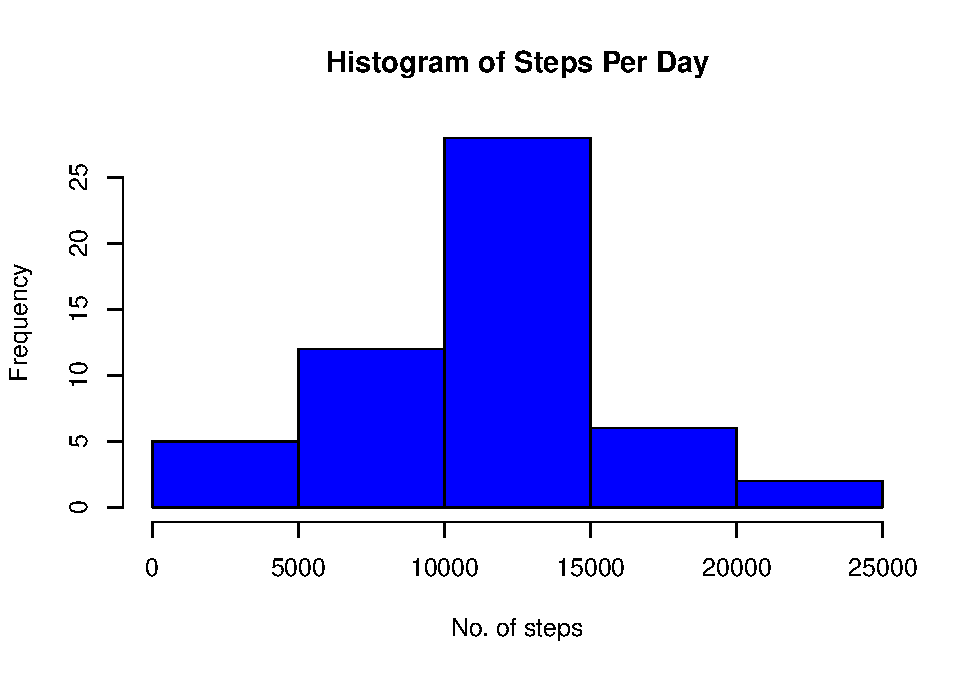
\includegraphics{PA1_template_files/figure-latex/unnamed-chunk-4-1.pdf}

\begin{enumerate}
\def\labelenumi{\arabic{enumi}.}
\setcounter{enumi}{2}
\tightlist
\item
  Calculate and report the mean and median of the total number of steps
  taken per day
\end{enumerate}

\begin{Shaded}
\begin{Highlighting}[]
\NormalTok{## Mean of the total number of steps taken per day}
\KeywordTok{mean}\NormalTok{(steps_perday}\OperatorTok{$}\NormalTok{steps)}
\end{Highlighting}
\end{Shaded}

\begin{verbatim}
## [1] 10766.19
\end{verbatim}

\begin{Shaded}
\begin{Highlighting}[]
\NormalTok{## Median of the total number of steps taken per day}
\KeywordTok{median}\NormalTok{(steps_perday}\OperatorTok{$}\NormalTok{steps)}
\end{Highlighting}
\end{Shaded}

\begin{verbatim}
## [1] 10765
\end{verbatim}

\subsection{What is the average daily activity
pattern?}\label{what-is-the-average-daily-activity-pattern}

\begin{Shaded}
\begin{Highlighting}[]
\NormalTok{avg_steps_int <-}\StringTok{ }\KeywordTok{aggregate}\NormalTok{(steps}\OperatorTok{~}\NormalTok{interval, activity, mean)}
\end{Highlighting}
\end{Shaded}

\begin{enumerate}
\def\labelenumi{\arabic{enumi}.}
\tightlist
\item
  Make a time series plot (i.e.~type = ``l'') of the 5-minute interval
  (x-axis) and the average number of steps taken, averaged across all
  days (y-axis)
\end{enumerate}

\begin{Shaded}
\begin{Highlighting}[]
\KeywordTok{plot}\NormalTok{(avg_steps_int}\OperatorTok{$}\NormalTok{interval, avg_steps_int}\OperatorTok{$}\NormalTok{steps, }\DataTypeTok{type =} \StringTok{"l"}\NormalTok{, }\DataTypeTok{main =} \StringTok{"Average steps taken per 5 minutes interval"}\NormalTok{, }\DataTypeTok{xlab =} \StringTok{"Interval (minutes)"}\NormalTok{, }\DataTypeTok{ylab =} \StringTok{"No. of Steps"}\NormalTok{)}
\end{Highlighting}
\end{Shaded}

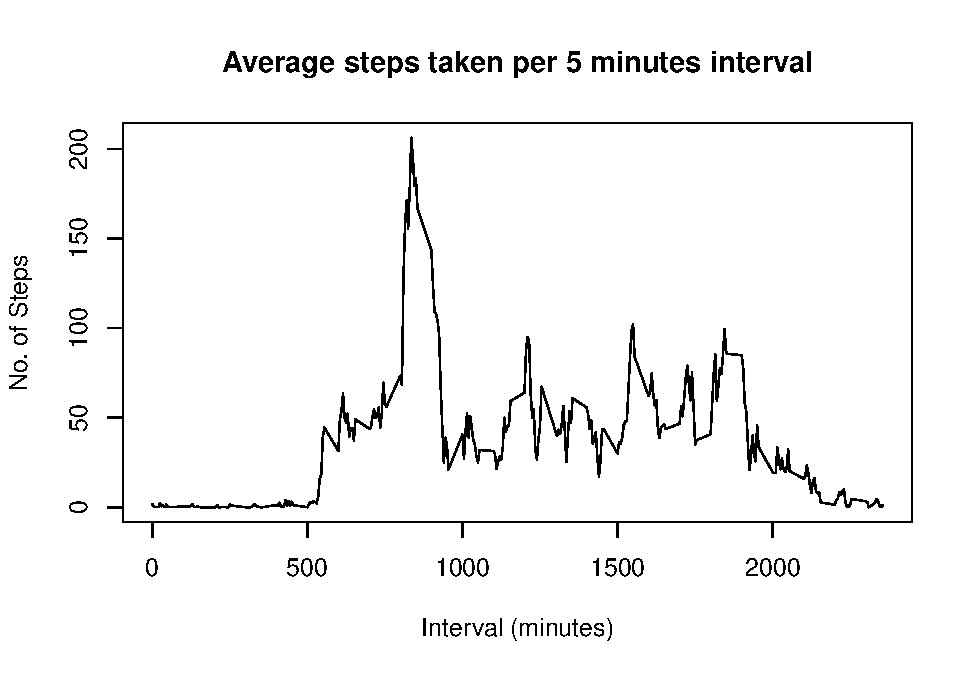
\includegraphics{PA1_template_files/figure-latex/unnamed-chunk-7-1.pdf}

\begin{enumerate}
\def\labelenumi{\arabic{enumi}.}
\setcounter{enumi}{1}
\tightlist
\item
  Which 5-minute interval, on average across all the days in the
  dataset, contains the maximum number of steps?
\end{enumerate}

\begin{Shaded}
\begin{Highlighting}[]
\NormalTok{## Get the max value index and print interval value}
\KeywordTok{cat}\NormalTok{(}\StringTok{"Interval "}\NormalTok{, avg_steps_int}\OperatorTok{$}\NormalTok{interval[}\KeywordTok{which.max}\NormalTok{(avg_steps_int}\OperatorTok{$}\NormalTok{steps)], }\StringTok{" with max average of"}\NormalTok{, }\KeywordTok{max}\NormalTok{(avg_steps_int}\OperatorTok{$}\NormalTok{steps), }\StringTok{" steps"}\NormalTok{)}
\end{Highlighting}
\end{Shaded}

\begin{verbatim}
## Interval  835  with max average of 206.1698  steps
\end{verbatim}

\subsection{Imputing missing values}\label{imputing-missing-values}

\paragraph{Note that there are a number of days/intervals where there
are missing values (coded as NA). The presence of missing days may
introduce bias into some calculations or summaries of the
data.}\label{note-that-there-are-a-number-of-daysintervals-where-there-are-missing-values-coded-as-na.-the-presence-of-missing-days-may-introduce-bias-into-some-calculations-or-summaries-of-the-data.}

\begin{enumerate}
\def\labelenumi{\arabic{enumi}.}
\tightlist
\item
  Calculate and report the total number of missing values in the dataset
  (i.e.~the total number of rows with NAs)
\end{enumerate}

\begin{Shaded}
\begin{Highlighting}[]
\KeywordTok{library}\NormalTok{(data.table)}

\NormalTok{activity <-}\StringTok{ }\KeywordTok{as.data.table}\NormalTok{(activity)}

\KeywordTok{nrow}\NormalTok{(activity[}\KeywordTok{which}\NormalTok{(}\KeywordTok{is.na}\NormalTok{(activity}\OperatorTok{$}\NormalTok{steps)),])}
\end{Highlighting}
\end{Shaded}

\begin{verbatim}
## [1] 2304
\end{verbatim}

\begin{enumerate}
\def\labelenumi{\arabic{enumi}.}
\setcounter{enumi}{1}
\tightlist
\item
  Devise a strategy for filling in all of the missing values in the
  dataset. The strategy does not need to be sophisticated. For example,
  you could use the mean/median for that day, or the mean for that
  5-minute interval, etc.
\end{enumerate}

\begin{Shaded}
\begin{Highlighting}[]
\NormalTok{avg_steps_interval <-}\StringTok{ }\KeywordTok{setnames}\NormalTok{(}\KeywordTok{data.table}\NormalTok{(}\KeywordTok{unique}\NormalTok{(activity}\OperatorTok{$}\NormalTok{date)),}\KeywordTok{c}\NormalTok{(}\StringTok{"date"}\NormalTok{))}
\NormalTok{avg_steps_interval <-}\StringTok{ }\KeywordTok{as.data.table}\NormalTok{(}\KeywordTok{aggregate}\NormalTok{(steps }\OperatorTok{~}\StringTok{ }\NormalTok{interval,}\DataTypeTok{na.rm =} \OtherTok{TRUE}\NormalTok{, }\DataTypeTok{data=}\NormalTok{activity, }\DataTypeTok{FUN=}\NormalTok{mean))}
\end{Highlighting}
\end{Shaded}

\begin{enumerate}
\def\labelenumi{\arabic{enumi}.}
\setcounter{enumi}{2}
\tightlist
\item
  Create a new dataset that is equal to the original dataset but with
  the missing data filled in.
\end{enumerate}

\begin{Shaded}
\begin{Highlighting}[]
\NormalTok{activity_clean <-}\StringTok{ }\KeywordTok{transform}\NormalTok{(activity, }\DataTypeTok{steps =} \KeywordTok{ifelse}\NormalTok{(}\KeywordTok{is.na}\NormalTok{(activity}\OperatorTok{$}\NormalTok{steps), }\DataTypeTok{yes =}\NormalTok{ avg_steps_interval}\OperatorTok{$}\NormalTok{steps, }\DataTypeTok{no =}\NormalTok{ activity}\OperatorTok{$}\NormalTok{steps))}
\end{Highlighting}
\end{Shaded}

\begin{enumerate}
\def\labelenumi{\arabic{enumi}.}
\setcounter{enumi}{3}
\tightlist
\item
  Make a histogram of the total number of steps taken each day and
  Calculate and report the mean and median total number of steps taken
  per day. Do these values differ from the estimates from the first part
  of the assignment? What is the impact of imputing missing data on the
  estimates of the total daily number of steps?
\end{enumerate}

\begin{Shaded}
\begin{Highlighting}[]
\NormalTok{steps_perday_clean <-}\StringTok{ }\KeywordTok{as.data.table}\NormalTok{(}\KeywordTok{aggregate}\NormalTok{(steps }\OperatorTok{~}\StringTok{ }\NormalTok{date, }\DataTypeTok{data=}\NormalTok{activity_clean, }\DataTypeTok{FUN=}\NormalTok{sum))}

\KeywordTok{hist}\NormalTok{(steps_perday_clean}\OperatorTok{$}\NormalTok{steps, }\DataTypeTok{col =} \StringTok{"blue"}\NormalTok{, }\DataTypeTok{xlab =} \StringTok{"Steps per day"}\NormalTok{, }\DataTypeTok{ylim =} \KeywordTok{c}\NormalTok{(}\DecValTok{0}\NormalTok{,}\DecValTok{30}\NormalTok{), }\DataTypeTok{main =} \StringTok{"Total number of steps per day"}\NormalTok{, }\DataTypeTok{breaks =} \KeywordTok{seq}\NormalTok{(}\DecValTok{0}\NormalTok{,}\DecValTok{25000}\NormalTok{,}\DataTypeTok{by=}\DecValTok{5000}\NormalTok{))}
\end{Highlighting}
\end{Shaded}

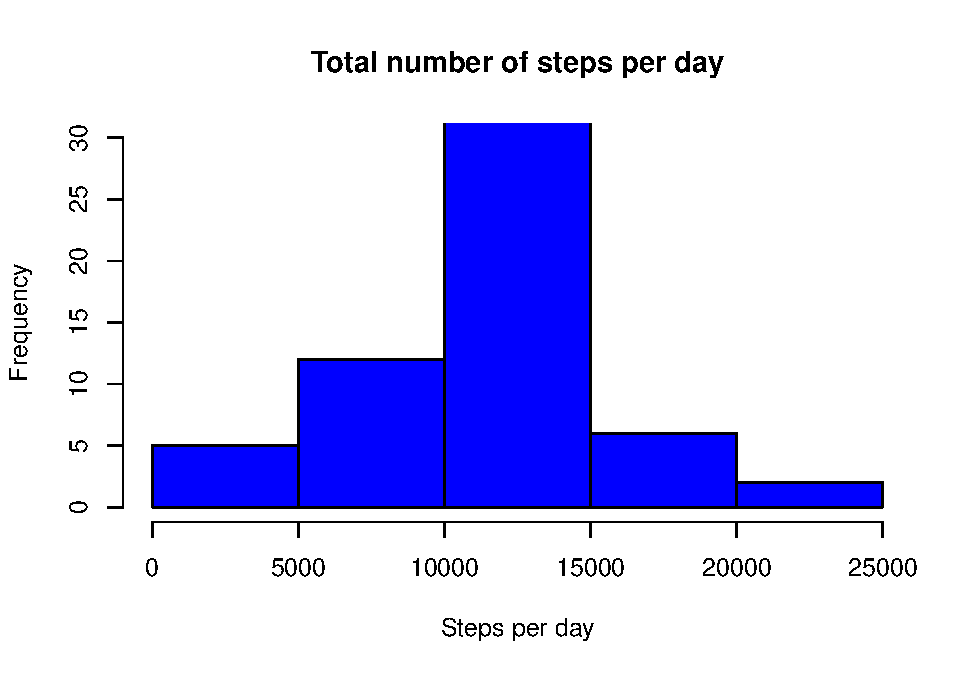
\includegraphics{PA1_template_files/figure-latex/unnamed-chunk-12-1.pdf}

\subsection{Are there differences in activity patterns between weekdays
and
weekends?}\label{are-there-differences-in-activity-patterns-between-weekdays-and-weekends}

\paragraph{For this part the weekdays() function may be of some help
here. Use the dataset with the filled-in missing values for this
part.}\label{for-this-part-the-weekdays-function-may-be-of-some-help-here.-use-the-dataset-with-the-filled-in-missing-values-for-this-part.}

\begin{enumerate}
\def\labelenumi{\arabic{enumi}.}
\tightlist
\item
  Create a new factor variable in the dataset with two levels -
  ``weekday'' and ``weekend'' indicating whether a given date is a
  weekday or weekend day.
\end{enumerate}

\begin{Shaded}
\begin{Highlighting}[]
\KeywordTok{library}\NormalTok{(chron)}
\end{Highlighting}
\end{Shaded}

\begin{verbatim}
## Warning: package 'chron' was built under R version 3.4.3
\end{verbatim}

\begin{Shaded}
\begin{Highlighting}[]
\NormalTok{activity_clean[}\KeywordTok{is.weekend}\NormalTok{(date),dayofweek}\OperatorTok{:}\ErrorTok{=}\StringTok{"Weekend"}\NormalTok{][}\OperatorTok{!}\KeywordTok{is.weekend}\NormalTok{(date),dayofweek}\OperatorTok{:}\ErrorTok{=}\StringTok{"Weekday"}\NormalTok{]}
\end{Highlighting}
\end{Shaded}

\begin{enumerate}
\def\labelenumi{\arabic{enumi}.}
\setcounter{enumi}{1}
\tightlist
\item
  Make a panel plot containing a time series plot (i.e.~type = ``l'') of
  the 5-minute interval (x-axis) and the average number of steps taken,
  averaged across all weekday days or weekend days (y-axis). See the
  README file in the GitHub repository to see an example of what this
  plot should look like using simulated data.
\end{enumerate}

\begin{Shaded}
\begin{Highlighting}[]
\NormalTok{activity_avg_clean <-}\StringTok{ }\KeywordTok{aggregate}\NormalTok{(steps}\OperatorTok{~}\NormalTok{interval }\OperatorTok{+}\StringTok{ }\NormalTok{dayofweek, activity_clean, mean, }\DataTypeTok{na.rm =} \OtherTok{TRUE}\NormalTok{)}
\NormalTok{plot<-}\StringTok{ }\KeywordTok{ggplot}\NormalTok{(activity_avg_clean, }\KeywordTok{aes}\NormalTok{(}\DataTypeTok{x =}\NormalTok{ interval , }\DataTypeTok{y =}\NormalTok{ steps, }\DataTypeTok{color =}\NormalTok{ dayofweek)) }\OperatorTok{+}
\StringTok{       }\KeywordTok{geom_line}\NormalTok{() }\OperatorTok{+}
\StringTok{       }\KeywordTok{labs}\NormalTok{(}\DataTypeTok{title =} \StringTok{"Average Steps taken by Day of Week"}\NormalTok{, }\DataTypeTok{x =} \StringTok{"Interval"}\NormalTok{, }\DataTypeTok{y =} \StringTok{"Average No. steps"}\NormalTok{) }\OperatorTok{+}
\StringTok{       }\KeywordTok{facet_wrap}\NormalTok{(}\OperatorTok{~}\NormalTok{dayofweek, }\DataTypeTok{ncol =} \DecValTok{1}\NormalTok{, }\DataTypeTok{nrow=}\DecValTok{2}\NormalTok{)}
\KeywordTok{print}\NormalTok{(plot)}
\end{Highlighting}
\end{Shaded}

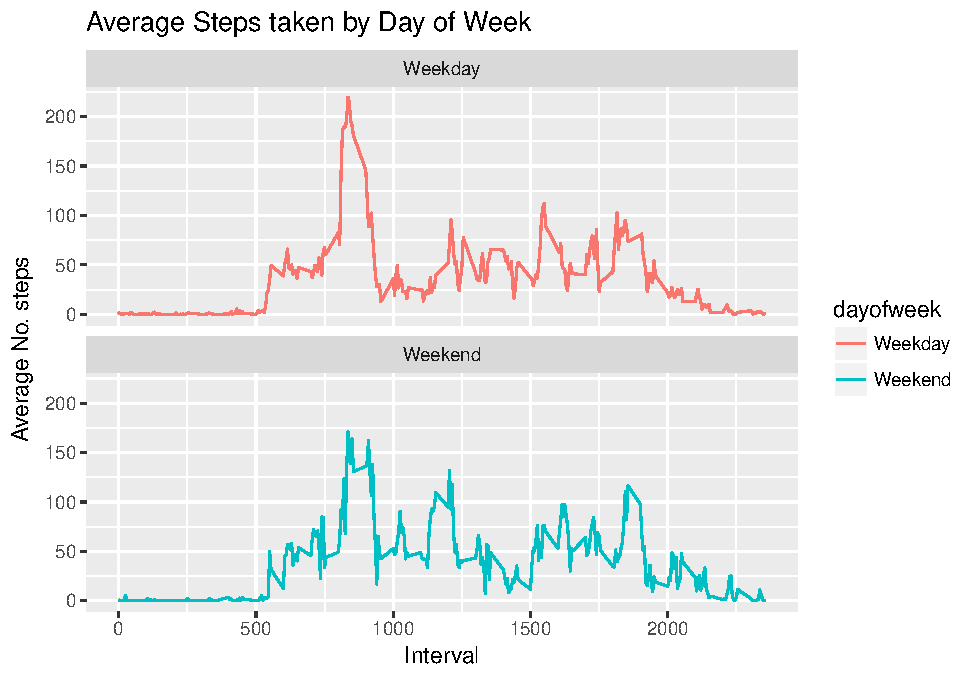
\includegraphics{PA1_template_files/figure-latex/unnamed-chunk-14-1.pdf}


\end{document}
